% ============================================================
% SHARED WORKSHOP BODY. Single source of truth for every workshop build's
% method, data, evaluation, limitations and conclusion sections. Edit this
% file once and every workshop PDF (World Models in Physical AI, and future
% workshops) changes together on the next compile.
%
% Kept deliberately venue-agnostic: no mention of a specific workshop's name
% or theme lives here. Per-workshop framing goes in the calling file
% (docs/paper/_workshop_<venue>.tex) via two connector macros expanded below:
%   \workshoprelatedworknote  - one bridging sentence at the end of Related
%                               Work, tying FactoryBench to that workshop's
%                               specific theme, right before the comparison
%                               table.
%   \workshopclosingnote      - one closing sentence at the end of the
%                               Conclusion, same purpose.
% A per-workshop file must \renewcommand these (defaults below are generic
% fallbacks so this file never hard-errors if used un-forked) and then
% \input this file after its own \maketitle / abstract / Introduction.
%
% NO APPENDIX HERE: this file ends at the bibliography, because most
% workshop CFPs cap pages "excluding references" with no appendix exemption.
% A venue whose CFP DOES exempt the appendix appends the shared
% ../paper/_appendix.tex in its own _workshop_<venue>.tex after inputting
% this file (see _workshop_physunderstanding.tex). Never add it here.
%
% PAGE BUDGET: as written this body runs ~6 pages, which fits an 8-page
% limit. A wrapper for a tighter venue sets \workshopcompacttrue (declared
% in _preamble_common.tex), which drops the three optional floats and the
% prose that depends on them, saving ~2 pages for a 6-page limit. Nothing
% load-bearing is gated: every claim and number survives compact mode, only
% the illustrative table/figure treatments are cut.
% ============================================================

% The two connector macros are declared in _preamble_common.tex, not here:
% a venue file is \input BEFORE this one, so a \providecommand at this point
% would run after the venue file had already renewed them, and be too late
% to define them.

\section{Related work}

Recent advances in LLM reasoning include prompting and deliberative strategies (e.g., Chain-of-Thought and Tree-of-Thought) \cite{wei2022chain,yao2023tree}, alongside tool-augmented paradigms such as Toolformer and ReAct \cite{schick2023toolformer,yao2023react,qin2023tool}. Time-series modeling has advanced through transformer-based architectures (Informer, Autoformer, FEDformer, PatchTST) \cite{zhou2021informer,wu2021autoformer,zhou2022fedformer,nie2022time}, strong alternative baselines such as TFT and N-BEATS \cite{lim2021tft,oreshkin2020nbeats}, and critical comparisons against simpler linear models \cite{zeng2023transformers}. Foundation-model directions (e.g., Chronos) explore transfer and zero/few-shot adaptation \cite{ansari2024chronos,das2024decoder}, with large-scale industrial corpora such as FactoryNet \cite{othman2026factorynetlargescaledatasetindustrial}, on which FactoryBench builds. Anomaly and reliability monitoring literature includes OmniAnomaly, USAD, and Deep SVDD \cite{su2019omni,audibert2020usad,ruff2018deep}, with surveys highlighting persistent gaps in interpretability and root-cause actionability \cite{chalapathy2019survey,lavin2015numenta}.

Causal frameworks provide formal tools for interventions and counterfactuals \cite{pearl2009causality,peters2017elements,rubin1974causal}, while temporal methods such as Granger causality and nonlinear causal discovery support directional reasoning in time series \cite{granger1969causal,runge2019causal}. \workshoprelatedworknote{}
\ifworkshopcompact
Against the closest Q\&A and time-series benchmarks (TimeSeriesExam~\cite{cai2024timeseriesexamtimeseriesunderstanding}, ChatTS~\cite{Xie_2025}, EngineMT-QA~\cite{wang2025itformerbridgingtimeseries}, Time-MQA~\cite{kong2025timemqatimeseriesmultitask}, QuAnTS~\cite{wenkel2024quants}, CLEVRER), FactoryBench is the only one that is simultaneously robot-grounded, multivariate, counterfactual, and accompanied by a new dense high-frequency dataset rather than relying exclusively on public or synthetic sources.
\else
Table~\ref{tab:benchmark_comparison} positions FactoryBench against closely related Q\&A and time-series benchmarks along eight axes; Counterfactual denotes Level~3 reasoning over alternative histories (Section~\ref{sec:levels}), Free-Form denotes open-ended answers scored by an LLM-as-judge voting protocol, and Novel Dense TS indicates whether the benchmark contributes a new high-frequency multivariate dataset rather than relying exclusively on public sources.
\fi

\ifworkshopcompact\else
\begin{table}[htbp]
    \centering
    \caption{Comparison of FactoryBench with existing benchmarks. ``Counterfactual'' = questions reasoning over alternative histories; ``Free-Form'' = open-ended answers judged by LLMs; ``Novel Dense TS'' = contributes a new multivariate high-frequency dataset.}
    \label{tab:benchmark_comparison}
    \small
    \resizebox{\textwidth}{!}{%
        \begin{tabular}{@{}lcccccccc@{}}
            \toprule
            Benchmark                    & \rotatebox{60}{Machine/Robot} & \rotatebox{60}{Multivariate TS} & Number of QAs & \rotatebox{60}{Counterfactual} & \rotatebox{60}{Ranking} & \rotatebox{60}{Numerical} & \rotatebox{60}{Free-Form} & \rotatebox{60}{Novel Dense TS} \\
            \midrule
            TimeSeriesExam               & \texttimes                    & \texttimes                      & $\sim$700     & \texttimes                     & \checkmark              & \texttimes                & \texttimes                & \texttimes                     \\
            ChatTS                       & \texttimes                    & \checkmark                      & $\sim$134k    & \texttimes                     & \checkmark              & \checkmark                & \texttimes                & \texttimes                     \\
            EngineMT-QA                  & \checkmark                    & \checkmark                      & $\sim$110k    & \texttimes                     & \checkmark              & \checkmark                & \checkmark                & \texttimes                     \\
            Time-MQA                     & \texttimes                    & \checkmark                      & $\sim$200k    & \texttimes                     & \checkmark              & \checkmark                & \checkmark                & \texttimes                     \\
            QuAnTS                       & \texttimes                    & \checkmark                      & $\sim$150k    & \texttimes                     & \checkmark              & \checkmark                & \checkmark                & \texttimes                     \\
            CLEVRER                      & \texttimes                    & \texttimes                      & $\sim$305k    & \checkmark                     & \texttimes              & \checkmark                & \checkmark                & \texttimes                     \\
            \midrule
            \textbf{FactoryBench (Ours)} & \checkmark                    & \checkmark                      & $\sim$71k     & \checkmark                     & \checkmark              & \checkmark                & \checkmark                & \checkmark                     \\
            \bottomrule
        \end{tabular}
    }
\end{table}
\fi

\section{FactoryBench framework}

\subsection{Four levels of machine understanding}
\label{sec:levels}

\ifworkshopcompact\else
\begin{table}[htbp]
    \centering
    \caption{FactoryBench levels, what they test, example questions, and expected answer formats.}
    \label{tab:levels_examples}
    \footnotesize
    \setlength{\tabcolsep}{4pt}
    \renewcommand{\arraystretch}{1.1}
    \begin{tabular}{@{}c l >{\raggedright\arraybackslash}p{4.6cm} >{\raggedright\arraybackslash}p{3.0cm} >{\raggedright\arraybackslash}p{1.7cm}@{}}
        \toprule
        Level      & Type           & Example question                                                                                                                                                 & What it tests                                                                   & Answer format \\
        \midrule
        \textbf{1} & State          & ``We want to isolate the lifting phase in the robot's time series. Assuming a fixed window length of 15 timesteps, at which timestamp should the window begin?'' & Can the model understand what the machine is doing and how it is behaving?      & Tensor        \\
        \textbf{2} & Intervention   & ``A collision with a foam cube occurs at $T{=}850$\,ms. Rank signal segments (A--D) in the order you would expect them to appear after the event.''              & Can the model reason about how the machine will behave in the face of an event? & Ranking       \\
        \textbf{3} & Counterfactual & ``Had a payload misconfiguration occurred at $T{=}200$\,ms, what would the target torque on joint~2 at $T{+}50$\,ms have been in this counterfactual case?''     & Can the model reason accurately about theoretical scenarios?                    & Scalar        \\
        \textbf{4} & Decision       & ``Given the sensor stream below, does the machine show signs of anomalous behavior? If yes, identify the root cause and the steps to fix it.''                   & Can the model make informed decisions about the machine?                        & Free-form     \\
        \bottomrule
    \end{tabular}
\end{table}
\fi

Our four-tier hierarchy builds on Pearl's ladder of causation association, intervention, and counterfactual reasoning, the organizing principle for causal inference and an increasingly common evaluation axis for machine-learning systems \cite{pearl2009causality,peters2017elements,jin2023cladder,pawlowski2020deep_scm,peyrard2020ladder}. We add a fourth decision-making level reflecting how industrial robotic platforms are actually operated: after interpreting state and causal relationships, operators must select and execute corrective procedures, typically prescribed by vendor manuals. This aligns with the diagnose-then-act loop standard in fault-tolerant control, and grounds each level in a qualitatively distinct reasoning skill with interpretable failure modes.

\textbf{Level 1: State.} Assesses the agent's ability to interpret the current state of the machine under normal conditions, including identification of operational modes and recognition of sensor patterns.

\textbf{Level 2: Intervention.} The agent must reason about the consequences of interventions or events occurring at the present timestep, including predicting the immediate impact of control actions and diagnosing emerging faults in real time.

\textbf{Level 3: Counterfactual.} Evaluates reasoning about hypothetical scenarios, requiring the agent to simulate alternative histories and assess how outcomes would differ under counterfactual conditions.

\textbf{Level 4: Decision Making.} The highest level evaluates the agent's ability to act on its understanding of the system: given a recorded episode and a task description, the agent must produce a diagnosis or remediation grounded in the previous three levels, reflecting what we expect from an LLM acting as an engineering assistant on the factory floor.

Each question is emitted in one of five answer formats (single-select MCQ, multi-select MCQ, ranking, tensor, free-form); the four structured formats are scored deterministically and free-form answers are scored by an LLM-as-judge voting protocol.

\subsection{Time series data and causal schema (SCE)}
\label{sec:sce}

So that the dataset structure itself encodes causality, all time-series signals are organized into three causal groups: \textbf{Setpoint} (the controller's commanded target), \textbf{Context} (physical and configured conditions), and \textbf{Effort+Feedback} (the machine's measured response). Under healthy operation the response is a known function of setpoint and context; faults manifest as structured residuals from that baseline, giving a single operational fault definition that applies across machines and tasks.

The data conforms to this schema across two source types: \textbf{FactoryWave}, a custom dataset generated from one-arm robotic platforms executing industrial tasks under varied conditions and systematically injected anomalies, and \textbf{open-source datasets} such as AURSAD~\cite{leporowski2022aursad} and voraus-AD~\cite{brockmann2023vorausad}, preprocessed to conform to the unified episode structure. All three sources provide the full setpoint--context--effort triplet at 83\,Hz or higher (Table~\ref{tab:datasets}).

\begin{table}[htbp]
    \centering
    \caption{Datasets incorporated into FactoryBench. FactoryWave is collected and released with this work; the other two are open-source datasets adapted to our schema. Tasks: PnP = pick-and-place, Scr = screwing, PiH = peg-in-hole.}
    \label{tab:datasets}
    \small
    \setlength{\tabcolsep}{4pt}
    \begin{tabular}{@{}l l c c c c@{}}
        \toprule
        Dataset                                & Robot          & Episodes & Frequency   & Tasks         & Anomalies \\
        \midrule
        AURSAD~\cite{leporowski2022aursad}     & UR3e           & 4094     & 100\,Hz     & Scr           & 4         \\
        voraus-AD~\cite{brockmann2023vorausad} & Yu-Cobot       & 2122     & 100/500\,Hz & PnP           & 12        \\
        FactoryWave (ours)                     & UR3, KUKA KR10 & 8983     & 125/83\,Hz  & PnP, Scr, PiH & 27        \\
        \bottomrule
    \end{tabular}
\end{table}

\section{Reliable Q\&A generation}

\subsection{Scalable generation via extensive labeling}

Scalable ground-truth generation is the central challenge of any Q\&A benchmark grounded in raw data. FactoryBench couples a structured labeling ontology with a context-free-grammar-style template system: each of the 21 templates contains variable slots filled at generation time either from label information read directly from the episode (signal names, timestamps, anomaly labels, root causes) or from a predefined sampling distribution attached to that slot (prediction horizons, thresholds, curated vocabularies). Answer options for single- and multi-select questions are drawn from a shared pool of pre-defined verifiable statements, each paired with a rule evaluated deterministically against the time series, so ground truth is never imputed but computed directly from the underlying labels; for single-select MCQ, the sampling step enforces that exactly one of the four options evaluates to true, so the question is unambiguous by construction. This is also our primary defense against template-generated benchmarks being solvable from surface structure alone: every template admits a combinatorially large instantiation space over signal names, timestamps, prediction horizons, and injected-fault types, so the correct answer is never recoverable from the question text alone and is always determined by the paired time series, which varies across instantiations. Alongside the full corpus we release \textbf{FactoryBench-Lite}, a $3{,}000$-item subset balanced across all $21$ templates and, within each template, on the dimension that determines its answer, so that a cheap evaluation is not weighted by how many items a template happens to contribute.

\subsection{Density of FactoryWave}
\label{sec:density}

\ifworkshopcompact\else
\begin{figure}[!h]
    \centering
    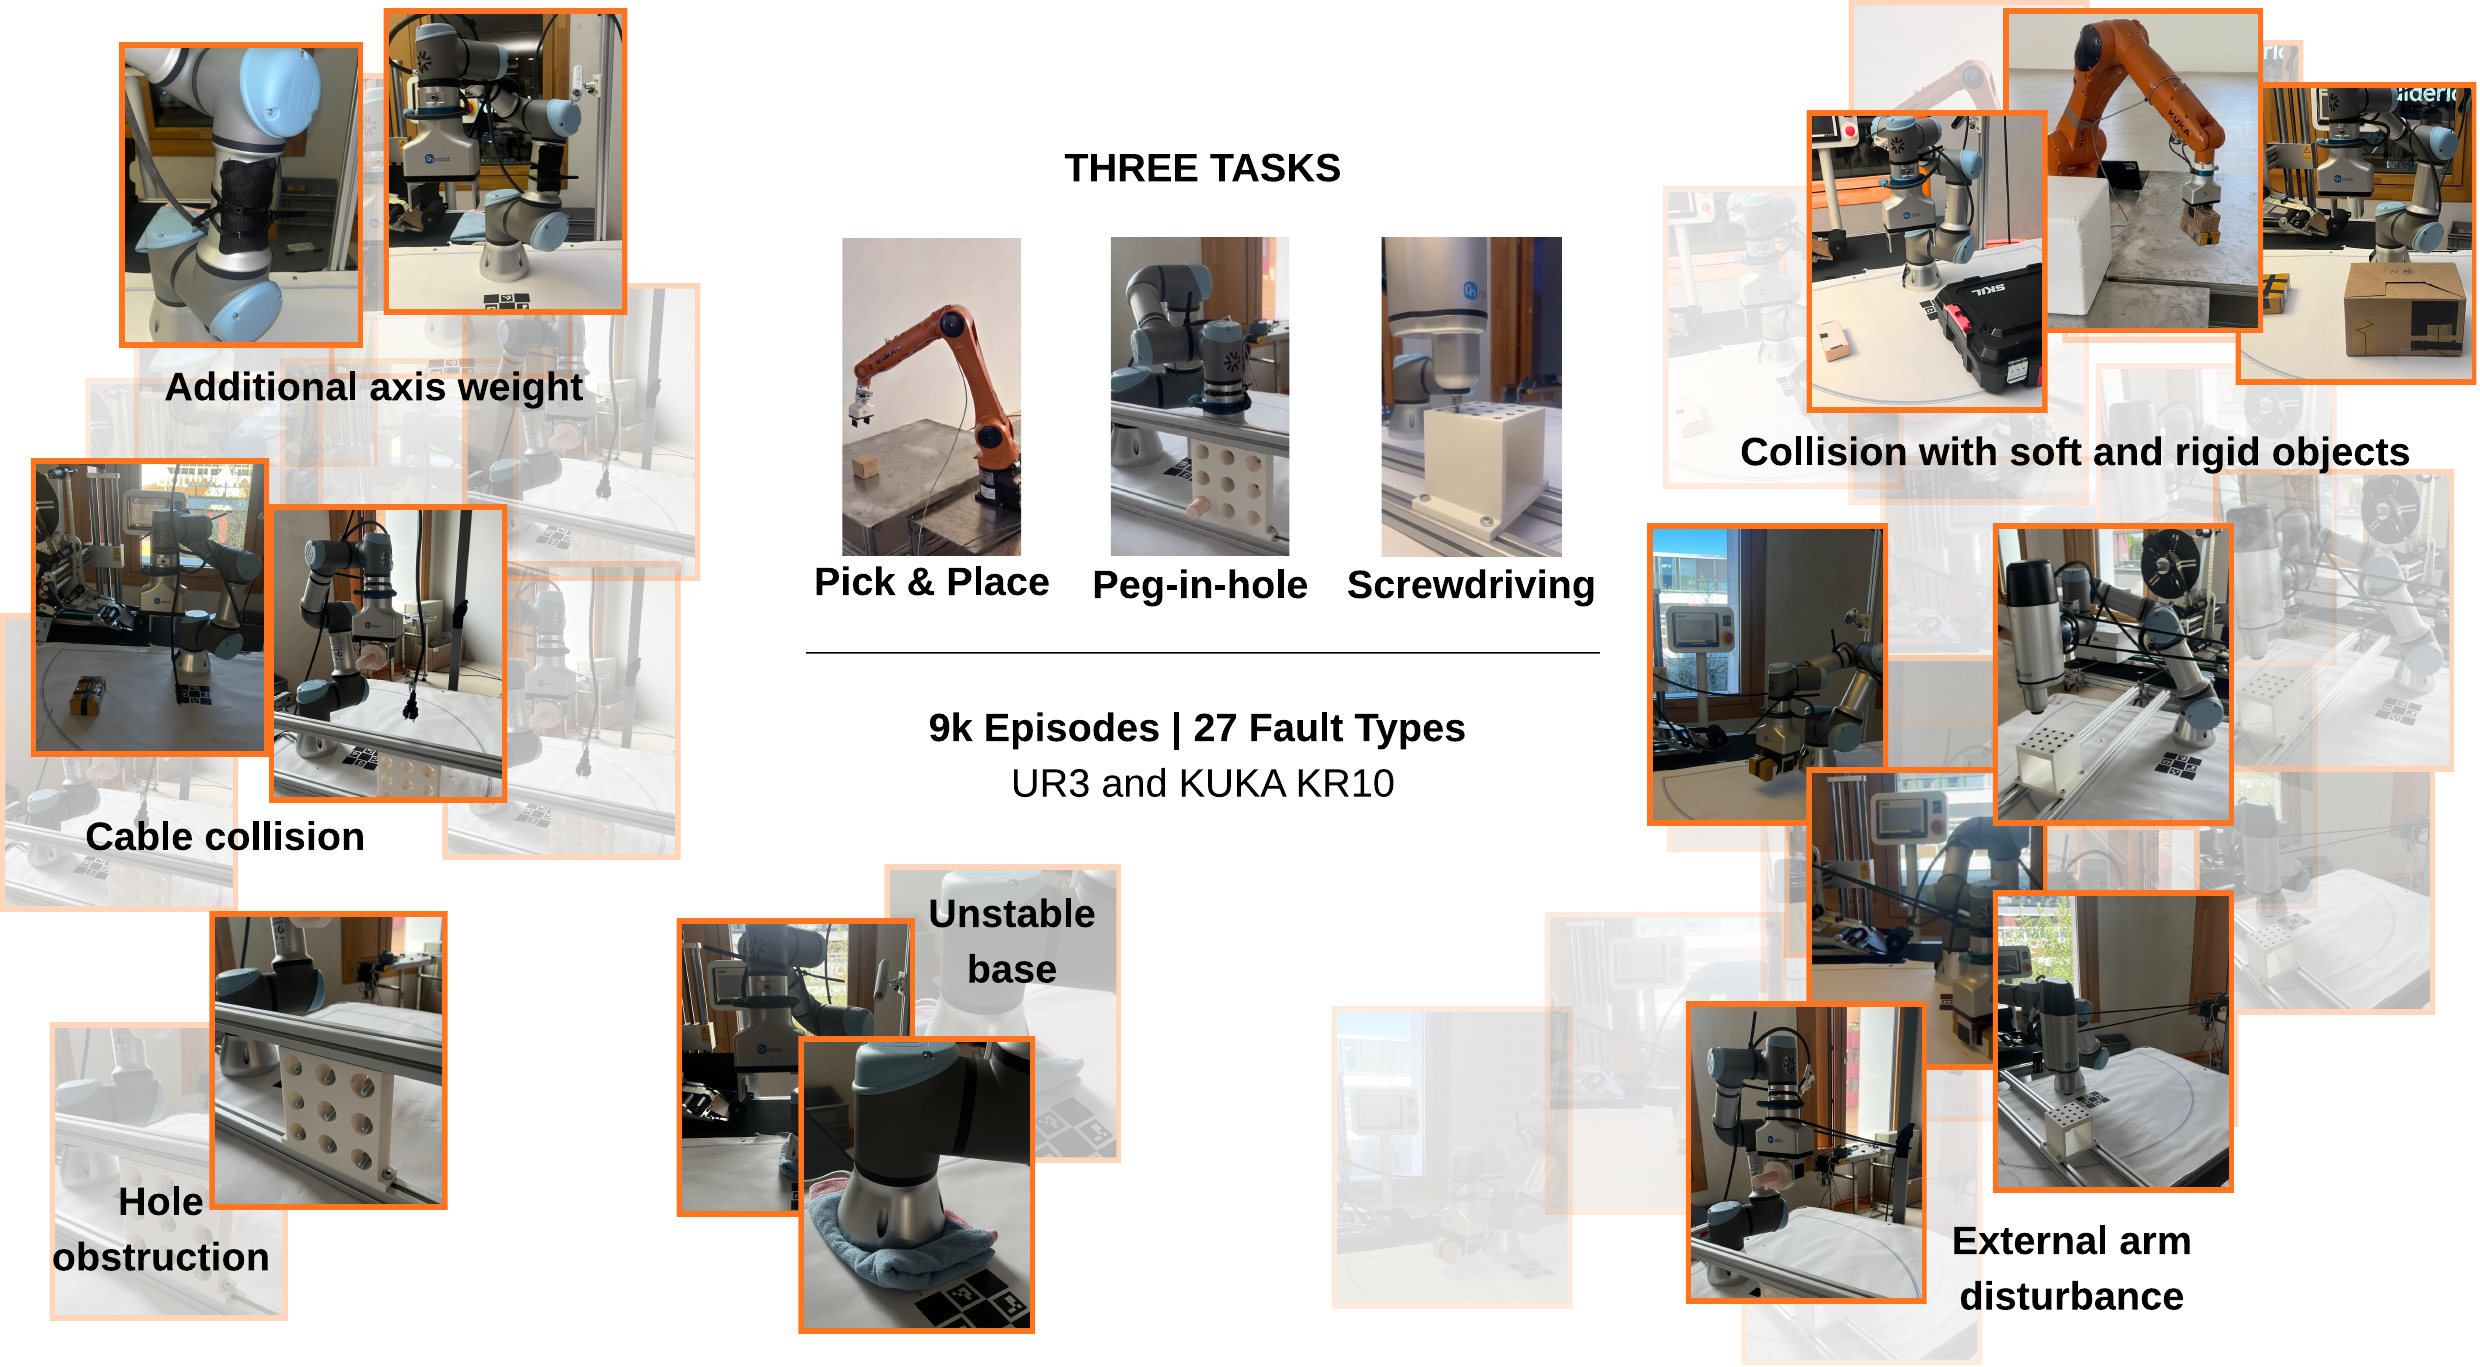
\includegraphics[width=\collagefrac\linewidth]{figures/factorybench-collage.pdf}
    \caption{FactoryWave tasks and fault catalogue. Photographs of the robotic platforms (UR3, KUKA KR10) executing the three tasks (pick-and-place, peg-in-hole, screwdriving) and a representative subset of the 27 systematically injected fault conditions.}
    \label{fig:factorywave_collage}
\end{figure}
\fi

FactoryWave is collected from two physical robots (UR3 and the KUKA KR10\ifworkshopcompact\else; Figure~\ref{fig:factorywave_collage}\fi) executing up to three industrial tasks each: pick-and-place, screwing, and peg-in-hole. Each complete task cycle constitutes one episode, recorded at 125 and 83\,Hz across over 100 sensor channels covering joint setpoints, feedback, torques, speeds, estimated contact forces, TCP pose, gripper state, and task-phase labels. To compensate for the limited tool-side telemetry exposed by the KUKA KSS controller, we additionally mount a 9-DoF inertial measurement unit on the KUKA gripper, streamed in sync with the controller signals.

Episodes are organized into three experiment types. \textbf{Normal} episodes capture nominal operation across three payload levels. \textbf{Fault} episodes inject one of 27 fault types (gripper failures, misconfigurations, collisions, and peg-in-hole-specific anomalies), each with fault-specific metadata and, where applicable, a precise injection timestep. \textbf{Counterfactual} episodes provide ground truth for Level~3 reasoning by approximating the do-operation on physical hardware: for each baseline we re-execute the task 3--5 times with every controllable condition held fixed and inject the target fault at a fixed timestep $t$, then keep the run whose pre-injection segment minimizes the signature kernel MMD against the baseline, using it as an approximate ground truth for hypothetical divergence.

\subsection{Knowledge graph and protocol extraction}
\label{sec:knowledge-graph}

Reliable ground truth for Level~4 troubleshooting requires machine-specific recovery protocols grounded in manufacturer documentation. For each robot we parse the manufacturer's official runtime error documentation into a structured mapping from error codes to descriptions and recommended recovery steps, then map every anomaly type in FactoryBench to the most likely corresponding manufacturer error code, with PhD-level robotics experts reasoning about the physical cause of each anomaly. Where a physical fault injection has no well-defined controller error, the same experts author the recovery protocol directly. The complete mapping is ingested into a knowledge graph alongside robot specifications, task definitions, and signal schema, which the generation pipeline queries at question-generation time to inject ground-truth protocol context into Level~4 items without per-question human review.

\section{Evaluation and results}

\subsection{Zero-shot evaluation}
\label{sec:zero-shot}

We evaluate a cross-vendor panel of frontier LLMs available at submission time (April 2026): Claude Sonnet 4.6 \cite{anthropic2025sonnet46} and GPT-5.1 \cite{openai2025gpt51} on the closed-weight side, and DeepSeek V3.2 \cite{deepseek2025v32}, Mistral Large 3 \cite{mistral2025large3}, and Qwen3-235B \cite{qwen2025qwen3} on the open-weight side, plus Qwen3-4B \cite{qwen2025qwen3} as a lightweight reference. For calibration we report a non-LLM baseline that dispatches per item by answer format: linear regression on the target signal for scalar and tensor templates, and uniform random over the option set for single- and multi-select MCQ and ranking templates (free-form Level~4 templates are excluded, as no traditional method maps cleanly to producing a remediation protocol). The panel is evaluated on FactoryBench-Lite, the balanced $3{,}000$-item subset described above, so that each level aggregate weights its templates equally instead of inheriting the episode pool's template mass; every model answers the identical items. Figure~\ref{fig:results} reports chance-corrected accuracy for the full panel.

\ifworkshopcompact
\begin{figure}[htbp]
    \centering
    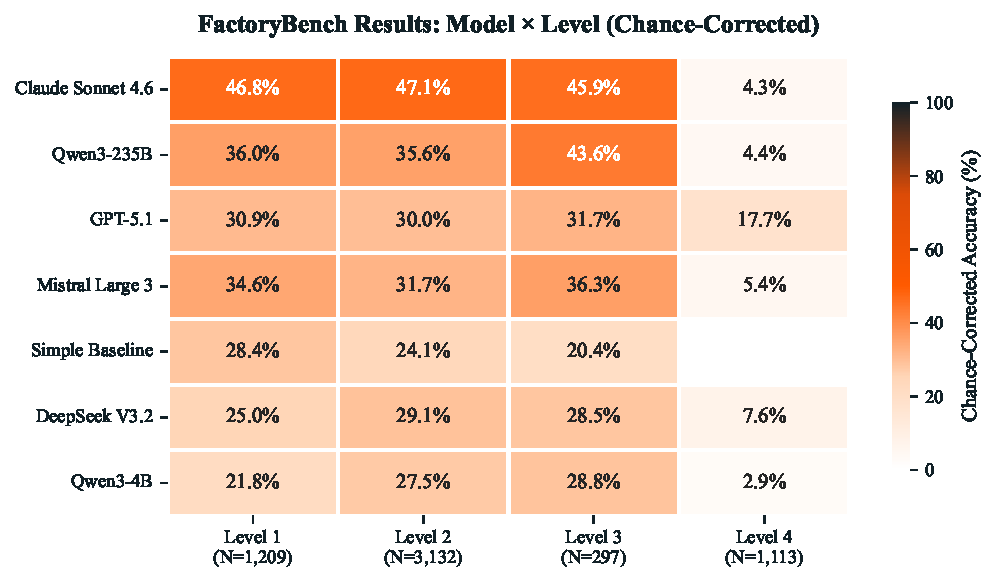
\includegraphics[width=0.82\linewidth]{../../output/figures/fig_main_heatmap.pdf}
    \caption{Main results: chance-corrected accuracy (\%) for the cross-model panel on FactoryBench's four reasoning levels.}
    \label{fig:results}
\end{figure}
\else
\begin{figure}[htbp]
    \centering
    \begin{subfigure}[t]{\linewidth}
        \centering
        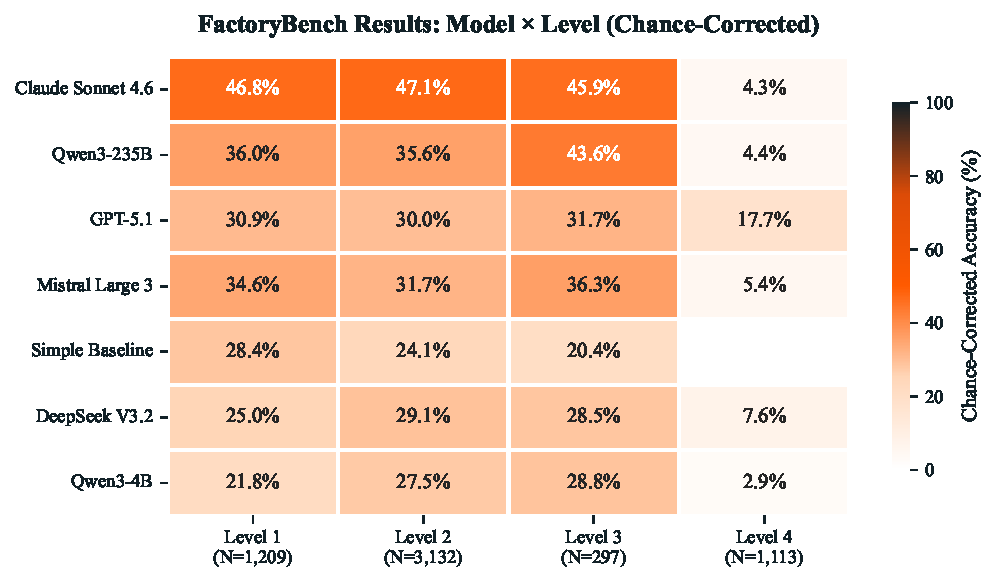
\includegraphics[width=\resultsafrac\linewidth]{../../output/figures/fig_main_heatmap.pdf}
        \caption{Chance-corrected accuracy (\%) on FactoryBench's four reasoning levels.}
        \label{fig:results-heatmap}
    \end{subfigure}\\[0.5em]
    \begin{subfigure}[t]{\linewidth}
        \centering
        \makebox[\linewidth][c]{
\includegraphics[width=\resultsbfrac\linewidth]{figures/fig_l4_gpt51_byrootcause.pdf}}
        \caption{GPT-5.1 L4 score distribution by ground-truth root cause (left, troubleshooting) and misconfigured parameter (right, optimization). Each bar shows the proportion of items scored 0/0.5/1; the right-edge value is the per-category mean accuracy.}
        \label{fig:results-gpt51-l4}
    \end{subfigure}
    \caption{Main results. \textbf{(a)} Cross-model panel performance across all four reasoning levels. \textbf{(b)} Per-fault and per-parameter breakdown of the GPT-5.1 L4 mass.}
    \label{fig:results}
\end{figure}
\fi

\subsection{Signal comprehension across Levels 1--3}

\paragraph{Most models fail to separate from the simple baseline on Level~1, including the largest in the panel.}
Under the signed chance correction the non-LLM baseline lands at $+4.3\%$ on L1. Four of six LLMs fail to clear it: Qwen3-4B ($-1.8\%$) and DeepSeek V3.2 ($-0.3\%$) score below chance outright, and GPT-5.1 ($+3.2\%$) and Qwen3-235B ($+3.6\%$) sit below the baseline despite being the largest models in the panel. Only Mistral Large 3 ($+5.9\%$) and Claude Sonnet 4.6 ($+11.8\%$) clear it, and Mistral only barely. Raw scale does not reliably confer the ability to extract precise state from dense industrial signals.

\paragraph{Models that struggle on Level~1 still outperform the baseline on Levels~2 and~3, and rank order is stable across the three.}
DeepSeek V3.2 ($+5.8\%$, $+17.1\%$) and GPT-5.1 ($+6.9\%$, $+27.5\%$) both lift clear of the L2/L3 baseline values ($-0.2\%$, $+6.2\%$) despite trailing it on L1, yet the model rank order is nearly identical across L1--L3: Claude Sonnet 4.6 leads at L2 and L3 ($+14.6\%$, $+45.7\%$), Qwen3-235B is the strongest open-weight model ($+20.6\%$ on L3), and Mistral Large 3 follows ($+5.3\%$, $+19.7\%$). This points toward state comprehension propagating into intervention and counterfactual reasoning rather than being substituted by it. The L3 margins carry one caveat: the trajectory-prediction template L3.5 awards the non-LLM baseline $+37.2\%$, which is not possible if that template's assumed chance level were correct, so part of every model's L3 figure reflects its scoring margin rather than counterfactual competence. We report L3 as measured rather than recalibrating, since changing the margin would redefine the metric and break comparability with the numbers released alongside the dataset.

\paragraph{A human expert reaches near-ceiling on Levels~1--2, but not on Level~3.}
\ifworkshopcompact
A robotics expert answered a $60$-item sample under open-tool, no-LLM conditions, graded by the benchmark's own scorer, reaching $0.962$ at L1 and $0.980$ at L2 against $0.712$ and $0.662$ for the strongest model: the gap is not an artifact of ambiguous items, and reading the signal out is what the panel fails at. At L3 the expert reaches only $0.625$ and does not lead the panel, which we attribute to counterfactual prediction being poorly served by existing tooling rather than to defective items.
\else
A robotics expert answered a $60$-item sample under open-tool, no-LLM conditions, graded by the benchmark's own scorer. On raw scores over the identical items the expert reaches $0.962$ at L1 and $0.980$ at L2, against $0.712$ and $0.662$ for the strongest model and $0.35$--$0.52$ for the rest: the gap is not an artifact of ambiguous items, the information is in the released signals, and reading it out is what the panel fails at. At L3 the expert reaches only $0.625$ and does not lead the panel, which we attribute to counterfactual prediction being poorly served by existing time-series tooling rather than to defective items.
\fi

\subsection{Engineering decision-making at Level 4}
\label{subsec:l4}

\paragraph{Level~4 exposes an industrial readiness gap, and the panel ordering reshuffles completely.}
On Level~4 (uncorrected 0/0.5/1 rubric, not directly comparable to the chance-corrected L1--L3 scores) the leader reaches 21.5\% and the other five score between 5.6\% and 19.9\%. Claude Sonnet 4.6, which leads L1--L3 and more than doubles the next model on L3, falls to fourth of six on L4 at 15.9\%. GPT-5.1 leads L4 at 21.5\%, and Qwen3-235B ($19.9\%$) and DeepSeek V3.2 ($17.8\%$) also overtake Claude Sonnet 4.6 there; L4 requires naming the root cause and producing a multi-step remediation grounded in manufacturer documentation, and we conjecture GPT-5.1's reversal reflects disproportionate pretraining exposure to structured industrial documentation, letting it match a protocol to a fault description even when its signal comprehension is weak. The dissociation between \emph{signal comprehension} and \emph{protocol retrieval} means optimizing for one does not deliver the other, and even models with strong L1--L3 comprehension either lack the machine-specific knowledge to diagnose faults, or cannot ground that knowledge in the observed signals. Closing this gap is the central challenge FactoryBench is designed to measure.

\paragraph{The L4 collapse is partly a read-out failure, not only a representational one.}
We probe this directly: linear probes on a frozen open-weight panel member recover fault \emph{presence} from the model's activations well above chance ($0.83$) even where the model's own answer stays below chance, whereas fault \emph{type} is only weakly decodable and no better than an untrained-network baseline. The information a correct L4 answer needs is thus partly already in the model's representations; part of what fails is turning it into a verbalized diagnosis, not only building it in the first place, a distinction that matters for whether better decoding, more grounding, or larger world models is the right fix.

% Compact builds drop this paragraph outright: it is the per-fault breakdown of
% Figure~\ref{fig:results-gpt51-l4}, and compact mode already omits that figure.
% This is the ONE place where compact mode loses content rather than just
% rewording, and it is needed to make a 6-page limit.
\ifworkshopcompact\else
\paragraph{GPT-5.1's L4 failures are asymmetric between troubleshooting and optimization.}
On troubleshooting ($n{=}143$, mean 0.189; Figure~\ref{fig:results-gpt51-l4}, left) the score distribution is sharply bimodal: 76.2\% zero, 14.0\% perfect, only 9.8\% partial. Because the evaluation subset draws root causes evenly, the perfects separate by fault physics rather than by class frequency: peg-insertion misalignment and rigid-object collision reach $0.67$, while every fault that changes assembly state without a mechanical transient (missing screw, extra component, loosening phase, unstable mounting) scores exactly $0.00$. On optimization ($n{=}143$, mean 0.241; Figure~\ref{fig:results-gpt51-l4}, right) GPT-5.1 scores perfectly exactly once and is the only model in the panel to do so at all: ground-truth answers are single-parameter corrections, but it emits lists of generic motion-tuning suggestions and treats payload configuration as one undifferentiated item among many, earning 0.5 at best. Even where GPT-5.1 leads L4, it remains weak at decision-making in an industrial context: it reaches $0.31$ on payload mass but only $0.04$ on TCP frame misconfiguration.
\fi

\subsection{Limitations}

\ifworkshopcompact
FactoryBench has three substantive limitations. Level~3 \emph{counterfactual} ground truth on hardware is approximate: two real runs cannot share an identical pre-injection state, so our signature-kernel-MMD-selected pair proxies the do-operation, and L3 scores conflate model reasoning with proxy quality. Our fault model is simplified, with atomic, fast faults drawn from a closed catalogue of 27 mechanisms rather than the compound, gradual faults of production, making this in-distribution fault \emph{recognition} more than the \emph{detection} problem operators face. And Level~4 ground truth comes from a finite catalogue of manufacturer codes and expert-authored procedures, so a model is partly evaluated on closed-book retrieval of protocols it may or may not have seen in pretraining.
\else
FactoryBench has three substantive limitations. Level~3 \emph{counterfactual} ground truth on physical hardware is fundamentally approximate: two real runs cannot share an identical pre-injection state, so our signature-kernel-MMD-selected pair is the closest empirical proxy for the do-operation rather than the do-operation itself, and L3 scores conflate model reasoning with proxy quality. As the first benchmark of its sort our fault model is simplified: industrial faults in production are typically compound and gradual, while ours are atomic, fast, and drawn from a closed catalogue of 27 injected mechanisms, making FactoryBench closer to in-distribution fault \emph{recognition} than the fault \emph{detection} problem operators actually face. Level~4 ground truth is drawn from a finite catalogue of manufacturer error codes and expert-authored recovery procedures, so a model is effectively evaluated on \emph{closed-book retrieval} of protocols it may or may not have seen during pretraining rather than on open-ended engineering reasoning, conflating ``does the model know this vendor manual?'' with ``can it reason from signals to a corrective action?''.
\fi

\section{Conclusion}

\ifworkshopcompact
We introduced FactoryBench, a four-level benchmark for machine understanding over industrial robotic telemetry, grounded in FactoryWave and structured around Pearl's causal hierarchy. Zero-shot evaluation of six frontier LLMs shows that signal comprehension and protocol-grounded decision-making do not co-develop: the L1--L3 ordering reshuffles entirely on L4, and structured-level scores stay well below 50\% (chance-corrected). \workshopclosingnote{} Extended results and protocols are released with the dataset and code (links above).
\else
We introduced FactoryBench, a four-level benchmark for machine understanding over industrial robotic telemetry, grounded in FactoryWave and structured around Pearl's causal hierarchy. Zero-shot evaluation of six frontier LLMs shows that signal comprehension and protocol-grounded decision-making are distinct capabilities that do not co-develop: the panel ordering on Levels~1--3 reshuffles on Level~4, with GPT-5.1 taking the L4 lead despite being mediocre on the structured levels while the L1--L3 leader ranks near the bottom on L4. Structured-level scores remain well below 50\% (chance-corrected) and no model approaches saturation on any level. \workshopclosingnote{} Full dataset details, extended per-format and per-robot breakdowns, the human-baseline protocol, and the full probing methodology are available in the extended paper and released alongside the dataset and code (links above).
\fi

% References begin on a fresh page. Every workshop build sits exactly at its
% CFP page limit, so letting the bibliography start halfway down the last body
% page makes it ambiguous whether that page counts as a main page. A clean
% break removes the question and reads better.
\clearpage
\bibliographystyle{\paperbibstyle}
\bibliography{../paper/references}
